\documentclass{article}
\usepackage{lipsum} % Paquete para texto de relleno
\usepackage{xcolor} % Paquete para colores
\usepackage{amsthm} % Paquete para teoremas y demostraciones
\usepackage{tikz} % Paquete para gráficos

\begin{document}
\textcolor{red}{Texto en rojo}

\lipsum[1] % Párrafo de texto de relleno
\newtheorem{theorem}{Teorema}[section] % Definición de teorema

\section{Introducción}
\begin{theorem}
Este es un teorema de ejemplo.
\end{theorem}
\begin{proof}
Esta es una demostración de ejemplo.
\end{proof}
Este ejemplo define un teorema y una demostración correspondiente.

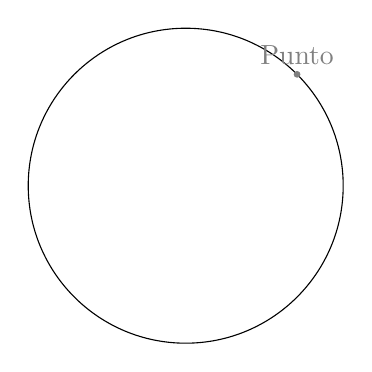
\begin{tikzpicture}
\draw (0,0) circle (2cm);
\filldraw[gray] (45:2) circle (1pt) node[above] {Punto};
\end{tikzpicture}
\end{document}